\chapter{Machine Learning Models Explored}

This section describes the structure of each machine learning models used for various gamma-ray spectroscopy tasks. The simplest model explored is the DNN. Because of the high dimension of the input data, feature extraction methods will be implemented and compared. These methods include PCA, a DAE, and a CAE. 

The other general architecture that will be explored is a 1D CNN. 


\section{Datasets Used for the Hyperparameter Search}

To show generalization improvements from including more physical parameters in the simulated dataset, the networks will be trained on two datasets. Because datasets of different complexity often need different architectures and hyperparameters \cite{Bergstra2012}, independent hyperparameter searches will be conducted for each dataset. The first dataset is comprised of unshielded gamma-ray spectra of ANSI isotopes simulated using GADRAS. Each spectrum has parameters randomly selected from Table \ref{table:hyperparameter_dataset_easy_parameters}. The average training error from 5-fold cross validation training using early stopping patience of 20 epochs was used to train 128 models. The maximum number of epochs was set to 200. A total of 1000 spectra are simulated for each isotope for the DNN. A total of 100 spectra are simulated for each isotope for the CNN due to computational constraints training the CNN.

\begin{table}[H]
\centering
\caption{Range of parameters used for the first hyperparameter search dataset.}
\label{table:hyperparameter_dataset_easy_parameters}
\begin{tabular}{c|c|c|}
\cline{2-3}
 & Hyperparameter Range & Sampling \\ \hline
\multicolumn{1}{|c|}{Source-Detector Distance {[}cm{]}} & 175.0 & N/A \\ \hline
\multicolumn{1}{|c|}{Source-Detector Height {[}cm{]}} & 100.0 & N/A \\ \hline
\multicolumn{1}{|c|}{FWHM 662 keV {[}s{]}} & 7.5 & N/A \\ \hline
\multicolumn{1}{|c|}{\begin{tabular}[c]{@{}c@{}}Shielding\\ (Percent 662 keV Attenuated)\end{tabular}} & 0\%, 20\% & Uniform \\ \hline
\multicolumn{1}{|c|}{Integration Time {[}s{]}} & 60 - 3600 & Uniform \\ \hline
\multicolumn{1}{|c|}{Linear Calibration Offset} & 0.8 - 1.2 & Uniform \\ \hline
\multicolumn{1}{|c|}{Signal to Background Ratio} & 0.5 - 2.0 & Uniform \\ \hline
\end{tabular}
\end{table}


\begin{table}[H]
\centering
\caption{Range of parameters used for the second hyperparameter search dataset.}
\label{table:hyperparameter_dataset_full_parameters}
\begin{tabular}{c|c|c|}
\cline{2-3}
 & Hyperparameter Range & Sampling \\ \hline
\multicolumn{1}{|c|}{Source-Detector Distance {[}cm{]}} & 50.5, 175.0, 300 & Uniform \\ \hline
\multicolumn{1}{|c|}{Source-Detector Height {[}cm{]}} & 50, 100.0, 150 & Uniform \\ \hline
\multicolumn{1}{|c|}{FWHM 662 keV {[}s{]}} & 7.0, 7.5, 8.0 & Uniform \\ \hline
\multicolumn{1}{|c|}{\begin{tabular}[c]{@{}c@{}}Shielding\\ (Percent 662 keV Attenuated)\end{tabular}} & 0\%, 20\%, 40\%, 60\% & Uniform \\ \hline
\multicolumn{1}{|c|}{Integration Time {[}s{]}} & 60 - 3600 & Uniform \\ \hline
\multicolumn{1}{|c|}{Linear Calibration Offset} & 0.8 - 1.2 & Uniform \\ \hline
\multicolumn{1}{|c|}{Signal to Background Ratio} & 0.5 - 2.0 & Uniform \\ \hline
\end{tabular}
\end{table}


\section{Hyperparameter Search Results}

The results of the hyperparameter searches are shown using random efficiency curves.

% These curves allow for reproducibility. These also allow for researchers who want to fit models to this dataset to have a performance benchmark. If you wanted to compare random hyperparameter search to more intelligent methods, you could compare using this.

\subsection{Dense Architecture}

Architecture and training hyperparamters are shown in Table \ref{table:hyperparameter_dataset_parameters_DNN}. Note, the number of nodes in each layers was made to decrease for each subsequent layer.

\begin{table}[H]
\centering
\caption{Range of hyperparameter explored for the DNN.}
\label{table:hyperparameter_dataset_parameters_DNN}
\begin{tabular}{c|c|c|}
\cline{2-3}
 & Hyperparameter Range & Sampling \\ \hline
\multicolumn{1}{|c|}{Number of Layers} & 1 - 3 & Uniform \\ \hline
\multicolumn{1}{|c|}{Nodes in Layer} & 2$^{5}$ - 2$^{10}$ & Power of Two \\ \hline
\multicolumn{1}{|c|}{Initial Learning Rate} & 10$^{-4}$ - 10$^{-1}$ & Logarithmic \\ \hline
\multicolumn{1}{|c|}{L2 Regularization Strength} & 10$^{-2}$ - 10$^{0}$ & Logarithmic \\ \hline
\multicolumn{1}{|c|}{Dropout Frequency} & 0 - 1 & Uniform \\ \hline
\multicolumn{1}{|c|}{Batch Size} & 2$^{4}$ - 2$^{10}$ & Power of Two \\ \hline
\multicolumn{1}{|c|}{Activation Function} & relu, tanh & Uniform \\ \hline
\multicolumn{1}{|c|}{Input Scaling} & sqrt, log1p & Uniform \\ \hline
\end{tabular}
\end{table}



Random efficiency curves for different reprocessing methods for the DNN are shown in Figure \ref{fig:random_hp_search_dnn_easy}. This figure implies that the optimum prepossessing step is BLANK. It's interesting that BLANK does better than BLANK.

\begin{figure}[H]
	\centering
	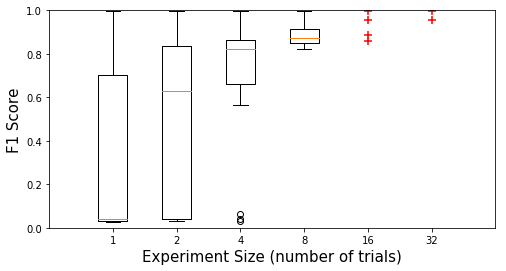
\includegraphics[width=0.8\linewidth]{images/random_hp_search_dnn_easy}
	\caption{Random hyperparameter search efficiency curves for the DNN using the first dataset.}
	\label{fig:random_hp_search_dnn_easy}
\end{figure}

\begin{figure}[H]
	\centering
	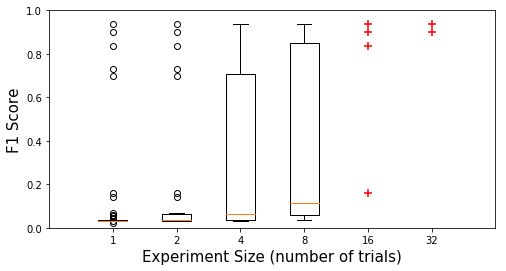
\includegraphics[width=0.8\linewidth]{images/random_hp_search_dnn_full}
	\caption{Random hyperparameter search efficiency curves for the DNN using the second dataset.}
	\label{fig:random_hp_search_dnn_full}
\end{figure}

In addition to hyperparameters associated with the DNN's architecture and training, hyperparameters explored include the autoencoder used. Autoencoders can generate a different encoding based on a given architecture. The mean squared reconstruction error may not be the best metric to measure how good this encoding is as a preprocessing step. To determine an optimum preprocessing architecture for the dense and convolutional autoencoder, the choice of preprocessing architectures was added as a hyperparameter. The choices belong to the set with the N best reconstruction errors, respective of dense and convolution architecture.

% \subsubsection{Hyperparameter Search Results - Autoencoders}

% Now that we know optimized autoencoder architectures for the DNN, we need to optimize training hyperparameters. 

% https://machinelearningmastery.com/activation-regularization-for-reducing-generalization-error-in-deep-learning-neural-networks/

% \cite{Ranzato2007} Fig 6 shows you can freeze the unsupervised feature extraction network and update the classifier if you have enough data.

% Sparse denoising autoencoders are included in in this work as feature extraction and dimension reduction techniques. Both autoencoders employ regularization techniques to ensure useful representations are learned. Both models includes $l1$ activity regularization as a method to induce sparsity on the networks activations, which increases generalization \cite{Goodfellow-et-al-2016}. 

% Show how well autoencoders worked at spectrum reconstruction and background subtraction. See if there's a large difference between doing background subtraction and 


\subsection{Convolution Architecture}

Just like the autoencoder, this can be done in one or two steps. One step: Train and optimize the entire network, convolution and dense layers. Two steps: Train and optimize the dense layer, using random initialization for non-trainable convolution filters. We'll probably go with the two-step.

\begin{table}[H]
\centering
\caption{Range of hyperparameter explored for the CNN.}
\label{table:hyperparameter_dataset_parameters_CNN}
\begin{tabular}{c|c|c|}
\cline{2-3}
 & Hyperparameter Range & Sampling \\ \hline
\multicolumn{1}{|c|}{Number of Filter Kernels} & \begin{tabular}[c]{@{}c@{}}(4)   (8)   (16)    (32)\\ (4, 8)  (8, 16)  (16, 32)\\ (4, 8, 16)   (8, 16, 32)\end{tabular} & Uniform \\ \hline
\multicolumn{1}{|c|}{Filter Kernel Length} & 2, 4, 8, 16 & Uniform \\ \hline
\multicolumn{1}{|c|}{Pooling size} & 2, 4, 8, 16 & Uniform \\ \hline
\multicolumn{1}{|c|}{Number of Dense Layers} & 1 - 3 & Uniform \\ \hline
\multicolumn{1}{|c|}{Nodes in Dense Layers} & 10 - 1000 & Logarithmic \\ \hline
\multicolumn{1}{|c|}{Initial Learning Rate} & 10\textasciicircum{}\{-4\} - 10\textasciicircum{}\{-1\} & Logarithmic \\ \hline
\multicolumn{1}{|c|}{L2 Regularization Strength} & 10\textasciicircum{}\{-2\} - 10\textasciicircum{}\{0\} & Logarithmic \\ \hline
\multicolumn{1}{|c|}{Dropout Frequency} & 0 - 1 & Uniform \\ \hline
\multicolumn{1}{|c|}{Batch Size} & 2\textasciicircum{}\{4\} - 2\textasciicircum{}\{6\} & Power of Two \\ \hline
\multicolumn{1}{|c|}{Activation Function} & tanh & Uniform \\ \hline
\multicolumn{1}{|c|}{Input Scaling} & sqrt, log1p & Uniform \\ \hline
\end{tabular}
\end{table}


\begin{figure}[H]
	\centering
	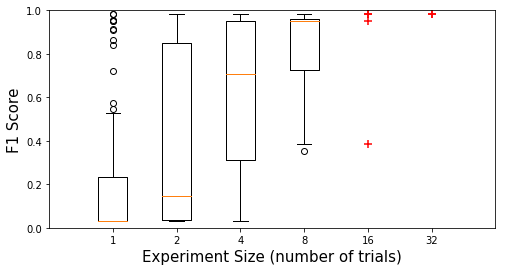
\includegraphics[width=0.8\linewidth]{images/random_hp_search_cnn_easy}
	\caption{Random hyperparameter search efficiency curves for the CNN using the first dataset.}
	\label{fig:random_hp_search_cnn_easy}
\end{figure}

\begin{figure}[H]
	\centering
	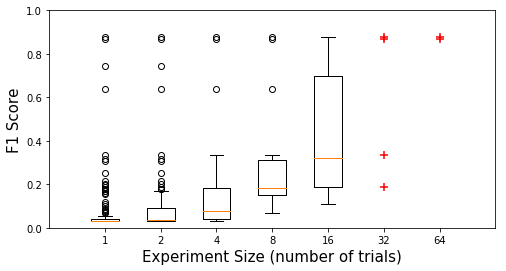
\includegraphics[width=0.8\linewidth]{images/random_hp_search_cnn_full}
	\caption{Random hyperparameter search efficiency curves for the CNN using the second dataset.}
	\label{fig:random_hp_search_cnn_full}
\end{figure}








\section{Summary of Final Model Architectures}

Learning curves are [definition, explanation]. Learning curves are used to determine a few things. We will use them to do [the following].

First, They are used as a sanity check, to make sure we are sampling our input space with enough granularity. To know we are sampling well enough, we should be sampling in a region where the curves are flat for both algorithms.

Secondly, Learning curves give us insight into which algorithm works better on the hyperparameter optimization dataset and simple version of the problem. We're expecting the CNN to outperform the DNN due to theoretical benefits of convolution architectures for our problem. We can also compare this curve to the final learning curves for the final datasets.



% Show learning curve to determine how many samples to add
\begin{figure}[H]
	\centering
	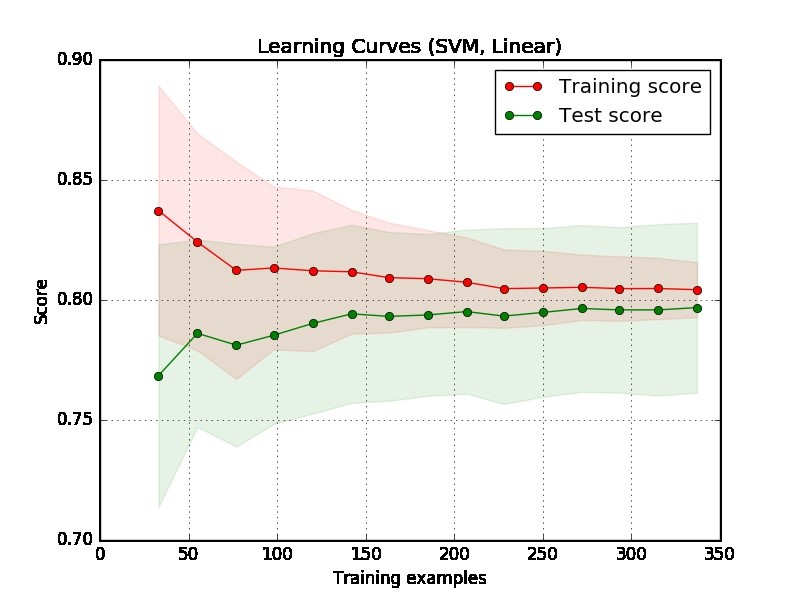
\includegraphics[width=0.8\linewidth]{model_choice_hyperparameter_search_images/learning_curve_dummy}
	\caption{Learning curves from the best DNN and CNN. X-axis will change to number of (input space sampling granularity? input space sampling divisions?). Shown: learning curve example.}
	\label{fig:Node}
\end{figure}








